%!TEX root = main.tex
% Tipo di documento. L'uso di twoside implica che i capitoli inizino sempre con la prima pagina a sinistra, eventualmente lasciando una pagina vuota nel capitolo precedente. Se questa cosa è fastidiosa, è possibile rimuoverlo. 
\documentclass[a4paper, twoside,openright]{report}
% \documentclass[a4paper,openright]{report}


\setcounter{secnumdepth}{4}
\setcounter{tocdepth}{4}

\usepackage{graphicx} % Required for inserting images
\setkeys{Gin}{width=0.6\columnwidth}

\usepackage[utf8]{inputenc}

\usepackage{hyperref}
\usepackage{adjustbox}

\usepackage{wrapfig}

\usepackage{enumitem}
\renewcommand{\labelitemi}{$\diamond$}
\renewcommand{\labelitemiii}{$\circ$}
\setlist[enumerate,2]{label=\roman*.}
\setlist[enumerate,3]{label=(\alph*)}

\setitemize{noitemsep}
\setenumerate{noitemsep}
\setlist{noitemsep}

\usepackage{paracol}
\usepackage{multicol}
\usepackage{booktabs}


\usepackage{geometry}

\usepackage{color}

\usepackage{listings}
% \usepackage{minted}

\usepackage{amsmath}
\usepackage{amssymb}
\usepackage{amsfonts}
\usepackage{mathtools}
\usepackage{bm}
\usepackage{nicefrac, xfrac}

\usepackage{wasysym}

% Uso dei colori
\usepackage[dvipsnames,table,xcdraw]{xcolor}
\usepackage{colortbl}
\usepackage{rotating}
\usepackage{adjustbox}

\usepackage{multirow}
\usepackage{booktabs}
\usepackage{makecell}


\usepackage{tikz}
\usetikzlibrary{automata, arrows,arrows.meta,bending}
\usetikzlibrary{positioning}
\usetikzlibrary{shapes.geometric}
\usepackage{parskip}
\usepackage{changepage}

\usepackage{soul}
\usepackage{cancel}

\usepackage{pifont} % used for tick \cmark and cross \xmark marks 

% This are needed because the correct double quotes would be ``'' or ``",
% but i've always written "text"
% TODO - check whether this affects listing environment
% \usepackage [english]{babel}
% \usepackage [autostyle, english = american]{csquotes}
% \MakeOuterQuote{"}

\usepackage{minitoc}

\geometry{margin=0.6in}

\setlist[description]{itemsep=0em,topsep=0.5em,parsep=0em}
\setlist[itemize]{itemsep=0em,topsep=0pt}
\setlist[enumerate]{itemsep=0em,topsep=0pt}

\hypersetup{
    colorlinks=true,
    linkcolor=black,
    filecolor=mauve,
    urlcolor=blue,
}

\definecolor{gray}{gray}{0.3}
\definecolor{verylightgray}{gray}{0.95}
\definecolor{blue}{rgb}{0,0,1}
\definecolor{mauve}{rgb}{0.58,0,0.82}
\definecolor{darkred}{rgb}{0.3,0,0}
\definecolor{darkgreen}{rgb}{0,0.3,0}
\definecolor{darkgray}{gray}{0.15}
\definecolor{lgray}{gray}{0.90}
\definecolor{darkorange}{RGB}{204,102,0}
\definecolor{darkviolet}{RGB}{85,0,170}



\newenvironment{notes}{
\par
\color{gray}
\small}

\newcommand{\note}[1]{\begin{notes}{#1}\end{notes}}
\newcommand{\nl}[0]{\parskip = \baselineskip}
\newcommand{\lst}[1]{\lstinline{#1}}
\newcommand{\ra}{\xrightarrow{\hspace*{2em}}}
\newcommand{\ns}{\setlength{\parskip}{0em}}

\newlength{\currentparindent}
\newcommand{\labelitemize}[2]{
\setlength{\currentparindent}{\parindent}
\setlength{\parindent}{0pt}

\begin{minipage}{0em} % Adjust the width as needed
    \makebox[0em][c]{\rotatebox{90}{\small #1}}
\end{minipage}
\begin{minipage}{\dimexpr\columnwidth-1cm\relax}
    #2
\end{minipage}
\setlength{\parindent}{\currentparindent}
}
\newcommand{\colfill}{\vspace{\fill}}

\newcommand{\framed}[1]{
\begin{center}
\fbox{
    \begin{minipage}{0.8\columnwidth}
        #1
    \end{minipage}
}
\end{center}}

\newcommand{\framedt}[2]{
\begin{center}
\fbox{
    \begin{minipage}{0.8\columnwidth}
        \vspace*{1em}
        \begin{center}
            \textbf{\ul{#1}}
        \end{center}
        \nl
        #2
    \end{minipage}
}
\end{center}}

\newcommand{\proscons}[4]{
    \begin{paracol}{2}
        \labelitemize{\color{darkgreen}\ul{\textit{#1}}}{
           \color{darkgreen}
           #3
        }
        \switchcolumn
        \labelitemize{\color{darkred}\ul{\textit{#2}}}{
           \color{darkred}
           #4
        }
     \end{paracol}
}

\newcommand{\coolquote}[2]{
    {
     \begin{center}
        \textit{\ul{``#1''}} --- #2
     \end{center}
	% \centering
}}

\newcommand{\textred}[1]{{\color{red}#1}}

\newcommand{\cmark}{\ding{51}}% TICK
\newcommand{\xmark}{\ding{55}}% CROSS

\newcommand\hcancel[2][black]{\setbox0=\hbox{$#2$}%
\rlap{\raisebox{.45\ht0}{\textcolor{#1}{\rule{\wd0}{1pt}}}}#2} 


\definecolor{pblue}{rgb}{0.13,0.13,0.8}
\definecolor{pgreen}{rgb}{0,0.5,0}
\definecolor{pred}{rgb}{0.9,0,0}
\definecolor{pgrey}{rgb}{0.46,0.45,0.48}

\lstset{frame=false,
 showstringspaces=false,
 breaklines=true,
%  columns=flexible,
 basicstyle={\small\ttfamily},
 keywordstyle=\color{blue},
 commentstyle=\color{darkgreen},
 stringstyle=\color{mauve},
 tabsize=2
}


\newtheorem{definition}{Definition}[chapter]
\newtheorem{theorem}{Theorem}[chapter]
\newtheorem{example}{Example}[section]


\usepackage{fancyhdr}
% \usepackage{nameref,autoref}

\pagestyle{fancy}
\fancyhf{}
\fancyhead[LE,RO]{\thepage} % Page number on Outer side of header on each page
\fancyhead[LO]{\leftmark} % section title on Left side of header on Odd pages
\fancyhead[RE]{\rightmark} % subection title on Right side of header on Even pages
\fancyfoot{}
\renewcommand{\headrulewidth}{0.4pt} % Width of line under the header
% \setcounter{secnumdepth}{2} % Depth of sectioning commands to include in the table of contents

% Rimuove il numero di pagina all'inizio dei capitoli
\fancypagestyle{plain}{
  \fancyfoot{}
  \fancyhead{}
  \renewcommand{\headrulewidth}{0pt}
}

\usepackage{emptypage}

\lstdefinelanguage{JavaScript}{
  keywords={typeof, new, true, false, catch, function, return, null, switch, var, if, in, while, do, else, case, break, for},
  keywordstyle=\color{pblue}\bfseries,
  ndkeywords={class, export, boolean, throw, implements, import, this, await},
  ndkeywordstyle=\color{pblue}\bfseries,
  identifierstyle=\color{black},
  sensitive=false,
  comment=[l]{//},
  morecomment=[s]{/*}{*/},
  commentstyle=\color{pgreen}\ttfamily,
  stringstyle=\color{purple}\ttfamily,
  morestring=[b]',
  morestring=[b]",
  morestring=[b]`,
  literate=
    {+}{{{\color{darkviolet}+}}}1
    % {-}{{{\color{darkviolet}-}}}1
    {*}{{{\color{darkviolet}*}}}1
    % {/}{{{\color{darkviolet}/}}}1
    {=}{{{\color{darkviolet}=}}}1
    {<}{{{\color{darkviolet}<}}}1
    {>}{{{\color{darkviolet}>}}}1
    {&}{{{\color{darkviolet}&}}}1
    {|}{{{\color{darkviolet}|}}}1
    {!}{{{\color{darkviolet}!}}}1
}
\lstset{
   language=JavaScript,
   backgroundcolor=\color{lgray},
   extendedchars=true,
   basicstyle=\footnotesize\ttfamily,
   showstringspaces=false,
   showspaces=false,
   numbers=left,
   numberstyle=\footnotesize,
   numbersep=9pt,
   tabsize=2,
   breaklines=true,
   showtabs=false,
   captionpos=b
}


% \titleformat{\chapter}[hang]{\vspace{-0em}\bfseries\Large}{}{0em}{\bf\Huge}

\lstset{language=JavaScript}


\definecolor{mybg}{RGB}{235, 231, 255}
\definecolor{mytext}{RGB}{24,0,156}

% Configure default style for listing blocks
\lstset{
  language=JavaScript
}

% Save original \verb command and redefine only \verb| syntax
\let\oldverb\verb

% Redefine \verb to use colorbox with custom styling
\makeatletter
\def\verb{\@ifnextchar|{\verb@colored}{\oldverb}}
\def\verb@colored|#1|{\colorbox{mybg}{\footnotesize\ttfamily\color{mytext}\detokenize{#1}}}
\makeatother

\title{MapReduce implementation in TypeScript \\{\large \textit{Scalable and Distributed Computing} Project}}
\author{Francesco Lorenzoni}
\date{October 2025}

\begin{document}

\maketitle
\tableofcontents

\chapter{Project Report}
% \lstset{language=JavaScript}

This is the report of the project developed for the ``Scalable and Distributed Computing'' course held at UniPi during the academic year 2024/25 by Prof. Dazzi.
The developed project consists of an implementation in TypeScript of the \textsc{MapReduce} framework, exploiting Kafka for message delivery and Docker for deployment.
The purpose was \textit{not} to develop a highly performant or resilient implementation of \textsc{MapReduce}; we have discussed other implementations, such as Hadoop and Spark, which work well and certainly would not be outperformed by a small project developed by a university student \smiley. \\
Instead, the intent was to define a problem whose resolution would lead to facing, from a practical point of view, some of the issues and concepts ---highlighted during lectures--- which arise when dealing with distributed applications.

\nl
\nl

This report will initially describe the main features and architecture of the implementation, and later discuss how it works under the hood and how it relates to the concepts discussed in the course.

\nl
\nl

{The course topics this project touches are:\ns
\begin{itemize}
   \item \ul{\textsc{MapReduce}}\\
   The project is a simple implementation of the \textsc{MapReduce} framework.
   \item \ul{\textit{Kafka and Distributed Messaging}}\\
   \textbf{Kafka} was chosen as the tool to share information among nodes, and to provide the messaging infrastructure. Kafka's design guided the messaging architecture, trying to exploit its \textit{publish-subscribe} and features at their best.
   \item \ul{\textit{Synchronizing}}\\
   Clearly some synchronization has to occur in a \textsc{MapReduce} framework. Making the nodes aware of when the pipeline of operations could proceed while keeping as little as possible \textbf{dependency} among them was one the main challenges of the development.
   Besides, to provide scalability, the synchronization mechanism could not rely on the number of active workers.
   \item \ul{\textit{BSP - Bulk Synchronous Paralle}l model}
   \textsc{MapReduce} can be seen as an instance of the \textbf{BSP} model, which helped to understand where the synchronization phase had to occur, and, subsequently how to properly design the synchronization mechanism.
   \item \ul{\textit{Scalability}}\\
   The implementation had to be \textbf{scalable}, allowing to add and remove workers dynamically. Kafka's design naturally allows consumers to go online and offline, but some parts of the implementation had to be designed with this in mind. The key point was keeping the synchronization mechanism not explicitly depending on the number of workers, but rather on the number of \textbf{partitions} per topic.
   \item \ul{\textit{CAP Theorem}}\\
   The CAP theorem tells us that in a distributed data store, it is impossible to simultaneously guarantee \textbf{consistency}, \textbf{availability}, and \textbf{partition tolerance}. This is relevant to our implementation, as we have to make some trade-offs between these properties when designing the messaging and synchronization architecture.\\
   More specifically, this led to have two slightly different implementations, trading off the properties in different ways. 
\end{itemize}}

\subsection*{Testing the implementation}
{\ns
\begin{lstlisting}[language=bash,literate={&}{{\&}}1]
   git clone git@github.com:frenzis01/MapReduceTS.git
   cd MapReduceTS
   # to clean output folder and remove old containers
   ./clean_output.sh && docker container prune -f && docker compose up
   # CTRL+C to stop the execution
   ./compare.sh # to compare distributed vs sequential results
\end{lstlisting}
\note{\footnotesize \texttt{source} nodes also compute the processing sequentially, allowing to compare the distribute MapReduce results with the sequential ones.}}
\newpage

\section{Abstract}
\begin{figure}[htbp]
   \centering
   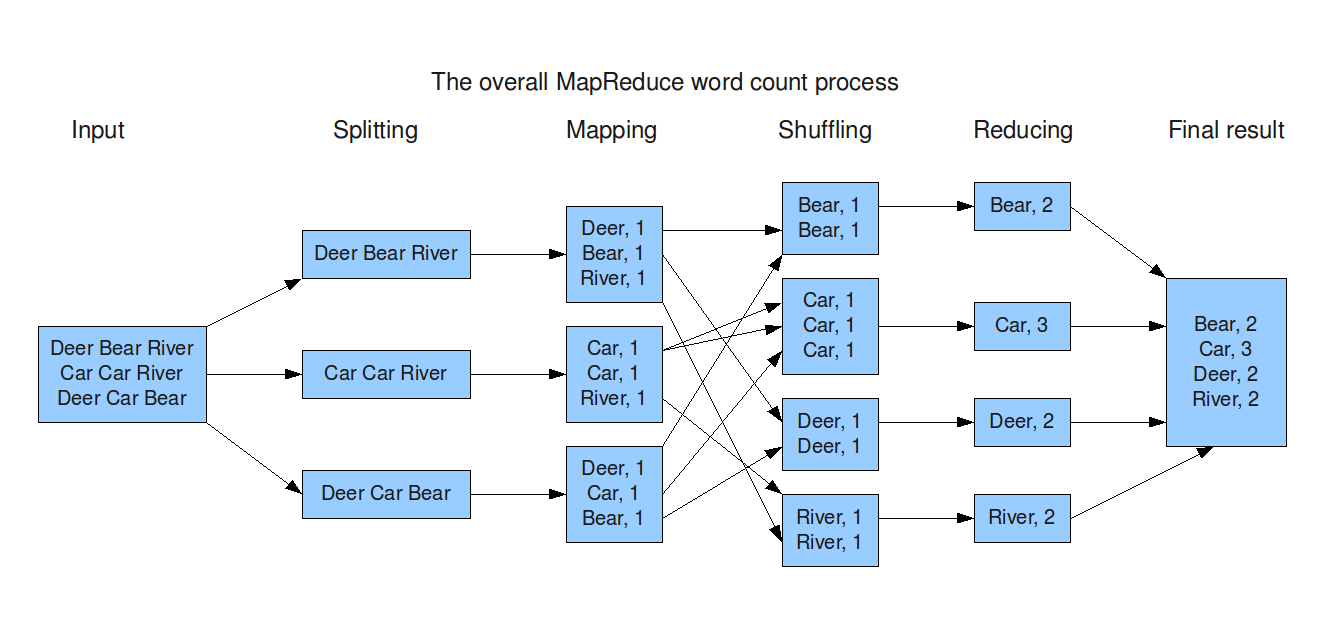
\includegraphics[width=\columnwidth]{images/mapreduce.png}
   \caption{MapReduce Word-Count schema}
   \label{fig:mapreduce}
\end{figure}

{MapReduce, as we have discussed it, during the lectures, includes the steps depicted in Fig. \ref{fig:mapreduce}, i.e.:\ns
\begin{enumerate} 
   \item Input/Splitting - Reading from an input source and parsing its content into data records.
   \item \textbf{Mapping} - \verb|map(k1,v1) -> [(k2,v2),...]| is a function that takes a pair of data and returns a list of pairs of new keys paired with values, and is applied in parallel to all input data.\footnote{\href{https://en.wikipedia.org/wiki/MapReduce}{wikipedia.org/MapReduce}}
   \item \textbf{Shuffling} - Shuffling consists of flattening the list of values \verb|[(k,v2), (k,v3), (k,v4), ...]| paired with a key \texttt{k} to get a pair like \verb|(k,[v2,v3,v4,...])|, preparing it for the reduce phase. In other words, shuffling's purpose is to distribute the key-value pairs to reducer nodes, preferably evenly. 
   \item \textbf{Reducing} - \verb|reduce(k2,[v2,...]) -> [(k3,v3),...]| is a function that takes a key and the related list of values and returns ---typically one or none--- pairs of keys and values. 
   \item Producing the result
\end{enumerate}}

\ul{The idea was to develop an implementation of MapReduce that allows the dynamic assignment of arbitrary \textit{``pipelines''} to generic worker nodes}. These pipelines consist of the \verb|map| and \verb|reduce| implementations for a given input data stream.\\
This means that the actual \verb|map| and \verb|reduce| functions are not hardcoded in the workers, but are instead defined by the user in a \texttt{source} node, which is responsible for gathering input data and defining the related pipelines.
Each worker simply knows its role in the architecture.

\section{Architecture}

\subsection{Nodes}
{This led the application to consist of the following five types(/roles) of nodes:\ns
\begin{enumerate}
   \item \texttt{source} - responsible for \ul{gathering input data} (from disk or elsewhere) and \ul{defining the related \texttt{map} and \texttt{reduce} functions} (the \textit{``pipeline''}, as it is referred to in the code), along with functions for selecting the key and the value from a data object, whose type and structure would be unknown to a worker.\\
   \texttt{source} nodes ---mostly--- ignore the underlying architecture of the MapReduce framework, \ul{they simply announce pipelines and send data records to a \texttt{dispatcher}}.\\
   \texttt{source} nodes are the ones to be \ul{defined by the user}, which have to obey some rules, but allow freedom regarding the actual MapReduce pipeline.
   \item \texttt{dispatcher} - receives data records from the source \ul{and distributes them to mappers}.
   \item \texttt{worker} - \ul{this implements either a \texttt{mapper}, a \texttt{shuffler} or a \texttt{reducer}}. The shuffling phase could also be performed as part of a \texttt{reducer} node, possibly improving performance and reducing message overhead, but it was kept separate for ``separation of concerns'' and to allow for possible more advanced load-balancing techniques for distributing records among reducer nodes.
   \item \texttt{sink} - \ul{receives the results} from the \texttt{reduce} and \ul{outputs them to disk}, or elsewhere. As with \texttt{source} nodes, this may be customized to suit the user's needs.
   \note{Clearly, the project includes basic implementations of \texttt{source} and \texttt{sink} nodes. }
\end{enumerate}}

\subsection{Message Passing}
\ul{The exchange of messages between nodes is managed by a \textbf{Kafka broker}}. 
Despite being the de-facto standard for distributed message passing, Kafka is \textit{not} ideally suited for big data streams or high-throughput applications.\\
It is not perfect from a performance standpoint, partly because the broker acts as both a single point of failure and a bottleneck. Nevertheless, it was chosen because its concepts of topics and partitions fit well with some of the communication requirements (and potential issues to solve) of the framework, and because ---based on how it was presented in the lectures--- it seemed an interesting tool to explore and learn.

{The Kafka topics architecture foresaw the following topics:\ns
\begin{itemize}
   \label{enum:simplerTopics}
   \item \verb|MAP_TOPIC|
   \item \verb|SHUFFLE_TOPIC|
   \item \verb|REDUCE_TOPIC|
   \item \verb|OUTPUT_TOPIC|
   \item \verb|PIPELINES_UPDATE_TOPIC| - Used for announcing new pipelines, allowing workers to get the \verb|map| and \verb|reduce| functions to execute on given data records.
\end{itemize}}

The functioning of Kafka topics and groups naturally allows for multiple workers belonging to a single \verb|'map-group'| to subscribe to \verb|'MAP_TOPIC'| and simultaneously consume messages from it; clearly, the same applies for all the other topics. 
Hence, \ul{we can dynamically add workers to the pool to scale our application, and the Kafka broker will automatically handle the distribution of messages among them}.

\begin{lstlisting}[caption={Sending MAP record to shuffle topic},label={lst:sendingMapRecord}]
   await producer.send({
      topic: SHUFFLE_TOPIC,
      // items with the same key will go to the same partition, i.e. the same shuffler
      messages: [{ 
         key: key, // key = keySelector(mapResult)
         value: JSON.stringify(newMessageValue(data, pipelineID)) // data = dataSelector(mapResult)
      }],
   });
\end{lstlisting}
Encoding the \verb|pipelineID| in the \verb|value| field allows us to distinguish the pipeline to which the data belongs; equivalently, we could also encode it and parse the \verb|key| field of a Kafka message, having something like \\ \verb|key: `${pipelineID}__map-record__{key}`|, but it's a less flexible and robust approach.\\
In this way, \ul{multiple data streams may be processed simultaneously with different} \verb|map| and \verb|reduce| \ul{functions for each of them}.

\section{Message retransmission issues}
\subsection{Kafka message retransmission}
Kafka consumers have an automatic mechanism for handling lost messages. Messages that have not been \textbf{committed} are \textbf{retransmitted} by the broker after some time. Hence, if a worker fails, another worker will resume the work it had left undone, based on the latest \texttt{offset} available for a given partition, which is incremented when \textit{committing} messages (automatically performed by Kafka consumers).

\subsection{Issues for lost messages}
Each pipeline (a tuple $\langle \texttt{PipelineID}, \texttt{map}, \texttt{reduce}, \texttt{keySelector}, \texttt{dataSelector} \rangle$) defined in a \texttt{source} node is encoded in a \verb|PipelineConfig| object, serialized as a string and later parsed in the workers.\\ 
Since pipeline updates are produced by \texttt{source} nodes and consumed by \texttt{worker}s in a dedicated topic (\verb|PIPELINES_UPDATE_TOPIC|), \ul{it may happen that the} \verb|PipelineConfig| \ul{object for a pipeline} \verb|P1| \ul{is not yet available when a \textit{data message}} (to be processed by either a \texttt{mapper} or a \texttt{reducer}) \ul{related to} \verb|P1| \ul{is received}, \ul{forcing the worker to add the message to a queue of ``not-yet-ready-to-be-processed'' messages}.\\
This is necessary because the worker needs to know the \verb|map| and \verb|reduce| functions in order to process a data record, which are defined in the \verb|PipelineConfig| object;
thus, in case the latter is not available, the worker cannot process the message and has to wait for it to be received.

If in this scenario the worker crashes for some reason, \ul{its messages pending to be processed are lost with it}.
They cannot simply get retransmitted by the Kafka Broker, because in the meantime some other messages related to ``ready'' pipelines $P_i \neq P_1$ would make the offset of the \verb|MAP_TOPIC| or \verb|REDUCE_TOPIC| progress.
So even manually handling the offset is not a viable solution.

\note{Instinctively it may seem appropriate to halt the worker until the \verb|PipelineConfig| object is available, to allow Kafka's retransmission system to work, but ---in case the \verb|PipelineConfig| is never received, or it is received after a long time--- this would lead to a performance drop, since the worker would not be able to process any other messages while waiting for the \verb|PipelineConfig| object.}

For this reason I attempted to develop \ul{an alternative and more intricate architecture for topics}, involving two \textbf{dynamically created topics} (\verb|MAP/REDUCE|) for each pipeline \verb|Pi|.
Having a topic for each data stream allows for separate message committing, hence \ul{avoiding the issue of lost messages}.

\subsection{Dynamic topics}
\note{This approach is implemented in the \texttt{multi-topic} branch of the repo.}

\ul{This implementation is error prone}. Error messages are displayed due to rebalancing, which is expected, but something else happens under the hood which I couldn't figure out, leading to message duplication and other issues.\\
Even though the code looked correct from a theoretical point of view, in practice something doesn't work out, possibly due to the approach attempting to stretch out too much Kafka's natural behavior.\\
Nevertheless, I still thought that a brief discussion on the idea behind this implementation could be interesting.  

The \texttt{dispatcher} node, upon receiving a new pipeline from a \texttt{source}, creates two topics specific for it:
\begin{lstlisting}
   [  topic: `${MAP_TOPIC}---${pipelineID}`,
      topic: `${REDUCE_TOPIC}---${pipelineID}`  ]
\end{lstlisting}

For what concerns \texttt{shuffler}s instead, since they do not need to compute either \verb|map| or \verb|reduce|, we can use a fixed unique \verb|`${SHUFFLE_TOPIC}`|, and encode the \verb|pipelineID| in the \verb|value| field of a message as displayed in \ref{lst:sendingMapRecord}.\\
Recall that \ul{\texttt{shuffler}s only need the \texttt{key} and the \texttt{pipelineID} to perform their job}, and these two are encoded in the \verb|key| and \verb|value| fields of a Kafka message, respectively. 

\texttt{mapper}s and \texttt{reducer}s have to \ul{subscribe to the topics dynamically created by the \texttt{dispatcher} while consuming other messages}. \\
This is in general \ul{\textit{not} trivial for Kafka}.\\
\verb|KafkaJS| does \textit{not} allow a consumer to subscribe to a topic while running and consuming messages.

{The only way to make consumers implement this mechanism appears to be:\ns
\begin{enumerate}
   \item \verb|stop()| the consumer 
   \item \verb|disconnect()| it from the broker
   \item \verb|connect()| again to the broker
   \item \verb|subscribe({newTopic})| to new topics
   \item \textit{start} (\verb|run(eachMessage: ...)|) consuming messages again
\end{enumerate}}
\note{Skipping disconnecting and reconnecting caused issues with duplicated messages and other weird behaviours.\\
This sequence seems instead to accomplish the goal, but not in every scenario.
}

Clearly, every time a worker performs these operations, a \textit{rebalance} is triggered, since the broker has to recompute the partition assignment to consumers of both the newly created topic and the ones to which consumers had already subscribed,
\ul{resulting in the application essentially halting for a few seconds}.

The \textbf{simpler approach} depicted earlier at \ref{enum:simplerTopics} \textbf{avoids this} and follows the more natural way of working for Kafka, where a consumer does not need to decide at runtime to which topics it should be interested in, or at least, decides ``only once'';
\ul{this comes at the cost of low fault tolerance concerning the handling of lost messages}.

\framedt{CAP theorem reminder}{
   The CAP theorem states that we can simultaneously have only two properties among \textit{Consistency}, \textit{Availability}, and \textit{Network Partitioning}. In our network-partitioned scenario, enforcing consistency leads to periods of unavailability, while guaranteeing (better) availability implies the possibility of ending up in an inconsistent state with some information lost.
}



\newpage
\section{Partitioning and Scalability}
\subsection{BSP model}
\begin{figure}[htbp]
   \centering
   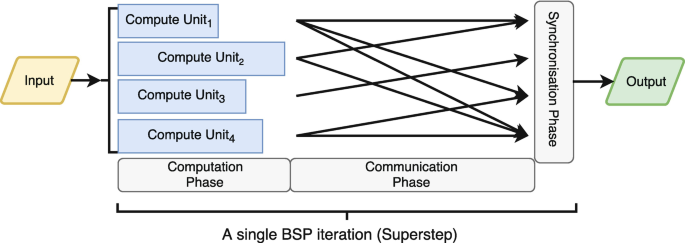
\includegraphics{images/bspmodel.png}
   \caption{BSP Model schema}
   \label{fig:bspmodel}
\end{figure}
BSP model is a way of thinking about distributed applications, which consists in dividing the application into \textit{supersteps}, where each superstep consists of a sequence of operations which are performed in parallel by the workers, followed by a synchronization phase where all the workers wait for each other to finish their superstep before proceeding to the next one.\\
In our case, synchronization occurs at the end of the computation \textit{map} records, and after they have been ``communicated'' to \texttt{shuffler}s. The keys for a given pipeline can be sent to the \texttt{reduce} only after all the \textit{map}s for that pipeline have been completed.
\framedt{Shuffling}{
   Since the shuffling process consists in putting map records into buckets, each bucket being a key, this happens as the map records are being consumed.\\
   Note that thanks to Kafka, \ul{records with the same key are always sent to the same partition}, hence they will be consumed by the same \texttt{shuffler} node, which will then be able to group them together.

   The shuffling phase can be considered over when there are no more \textit{map} records to be consumed. At that point, the \texttt{shuffler} nodes can start sending the \textit{shuffle} records to the \texttt{reduce} topic, which will be consumed by the \texttt{reducer} nodes.
}

\framedt{Reducing}{
   The \texttt{reducer} nodes can start consuming messages from the \texttt{reduce} topic as soon as they are available, and process them right away.
   This is because the \verb|reduce| operation needs only the list of values for a given key, which is all packed in a single \textit{shuffle} record, and does not depend on the completion of other \textit{reduce} operations.
   Besides, given that the \texttt{shuffler}s wait for all \textit{map} records to be consumed before sending the \textit{shuffle} records, we can be sure that all the \textit{map}s for a given key have been completed before the \textit{shuffle} record is sent to the \texttt{reduce} topic, so if a shuffle record is received, then we are \textit{sure} that all the \textit{map}s for that key have been completed and are in such \textit{shuffle} record.\\
   Note also that if a \texttt{reducer} receives the \textit{shuffle} record for a key $k_1$, \ul{it is guaranteed by Kafka that it is the only worker handling} $k_1$, so no duplicated processing will happen. 
}
The \texttt{sink} nodes instead, can simply start consuming messages from the \verb|OUTPUT_TOPIC| as soon as they are available, without waiting for all the \texttt{reduce} operations to finish.

\subsection{Implementation Key Points}

There are some key points concerning our implementation which we have to highlight:
\begin{itemize}
   \item There must be a special message to signal the end of \textit{source} records, so that the \textit{dispatcher} node knows when the data stream has ended.
   \item The \textit{dispatcher} has to propagate the end of the source data stream to all the \textit{map} nodes, so that they know when to propagate the end-of-stream message to the \textit{shuffle} nodes.
   \item There must be special messages to signal the end of \textit{map} records, so that the \textit{shuffle} nodes know when they can start feeding the reduce nodes.
   \item The special messages will have a special \verb|key| and a special \verb|value|.
   \item Topics are divided into partitions, which are the basic unit of parallelism in Kafka. Each partition is consumed by a single worker, but a single worker can consume multiple partitions.
   \item The partition to which a message is sent is determined by the \verb|key| of the message, which is hashed to determine the partition. This means that messages with the same key will always be sent to the same partition, and hence will be consumed by the same worker.
   \item Partitions indicate the degree of parallelism of the application, i.e. how many workers can consume messages from a topic at the same time.
\end{itemize} 

\subsection{Ending the Stream}
The end of the stream is signaled by a special message with a special key and value, which is sent by the \texttt{source} node to the \texttt{dispatcher}.
\begin{lstlisting}[label={lst:streamEndedSource},caption={Sending STREAM\_ENDED message from source to dispatcher},captionpos={top}]
   await producer.send({
      topic: DISPATCHER_TOPIC,
      messages: [{
         key: `${pipelineID}__${STREAM_ENDED_KEY}`,
         value: JSON.stringify(newStreamEndedMessage(pipelineID, data.length)),
      }],
   });
\end{lstlisting}
 
The dispatcher will then forward this message to all the \textit{map} nodes, which will then propagate it to the \textit{shuffle} nodes, which will then propagate it to the \textit{reduce} nodes, and finally to the \texttt{sink} nodes.\\
However, \ul{there is a major problem which must be addressed} and discussed, before talking about the solution. \ul{A message with this key} \verb|`${pipelineID}__${STREAM_ENDED_KEY}`|, \ul{will only be received by \textit{exactly one} map consumer}, so there must be some way to either propagate or distribute it among the consumers.

\subsubsection{Partitions for message propagation}
\ul{It is crucial for a proper distributed and scalable architecture to allow adding and removing workers, so the propagation \textit{cannot} rely on workers knowing each other or making assumptions about the cluster topology.}\\
To solve this we can use a \textbf{fixed} explicit number of partitions per topic, such as 10. This will represent the maximum number of workers that can consume messages from a topic at the same time, so having more workers than partitions will not lead to performance improvements.
This will be one of the few data structures shared among nodes.
\note{The number of partitions can be adjusted by the user to fit the needs of the application.} 

\begin{lstlisting}[label={lst:bucketsize},caption={BUCKET\_SIZE represents the number of partitions per topic.},captionpos={top}]
for (let i = 0; i < BUCKET_SIZE; i++) {
      await producer.send({
         topic: MAP_TOPIC,
         messages: [{
            key: `${pipelineID}__${STREAM_ENDED_KEY}`,
            value: JSON.stringify(newStreamEndedMessage(pipelineID, expectedMessages)),
            partition: i
         }],
      });
   }
\end{lstlisting}

We can send the message to all the partitions of the topic as depicted in Lst. \ref{lst:bucketsize}, so that it is guaranteed that all consumers will receive it. If there are less workers than partitions, some of them will receive the message multiple times.\\
More details on handling \verb|STREAM_ENDED| messages are discussed in Sec. \ref{sec:streamEnding}, and in the scheme in Fig. \ref{fig:redisSynch}.

\subsubsection{Message ordering}
It is important to note that \ul{Kafka guarantees message ordering only within a partition}, not across partitions.
Here lies the reason why we can't have a \texttt{mapper} receiving the \textit{end of stream} message to propagate it to other mappers polling other partitions. It may happen that the propagated end message is received by a \texttt{mapper} before other remaining source records, which would lead to the \texttt{mapper} not processing them, and hence losing some data.\\
Hence, we must send a \verb|STREAM_ENDED| for each \verb|MAP_TOPIC| partition from the dispatcher after it has sent all the source records.
In this way, we are sure that in each partition the \verb|STREAM_ENDED| message is received after all the source records.

\newpage
\subsection{Wrap Up}
Below we have a scheme wrapping up the overall messaging architecture of the application, to display how the messages flow among the nodes.

\begin{figure}[htbp]
   \centering
   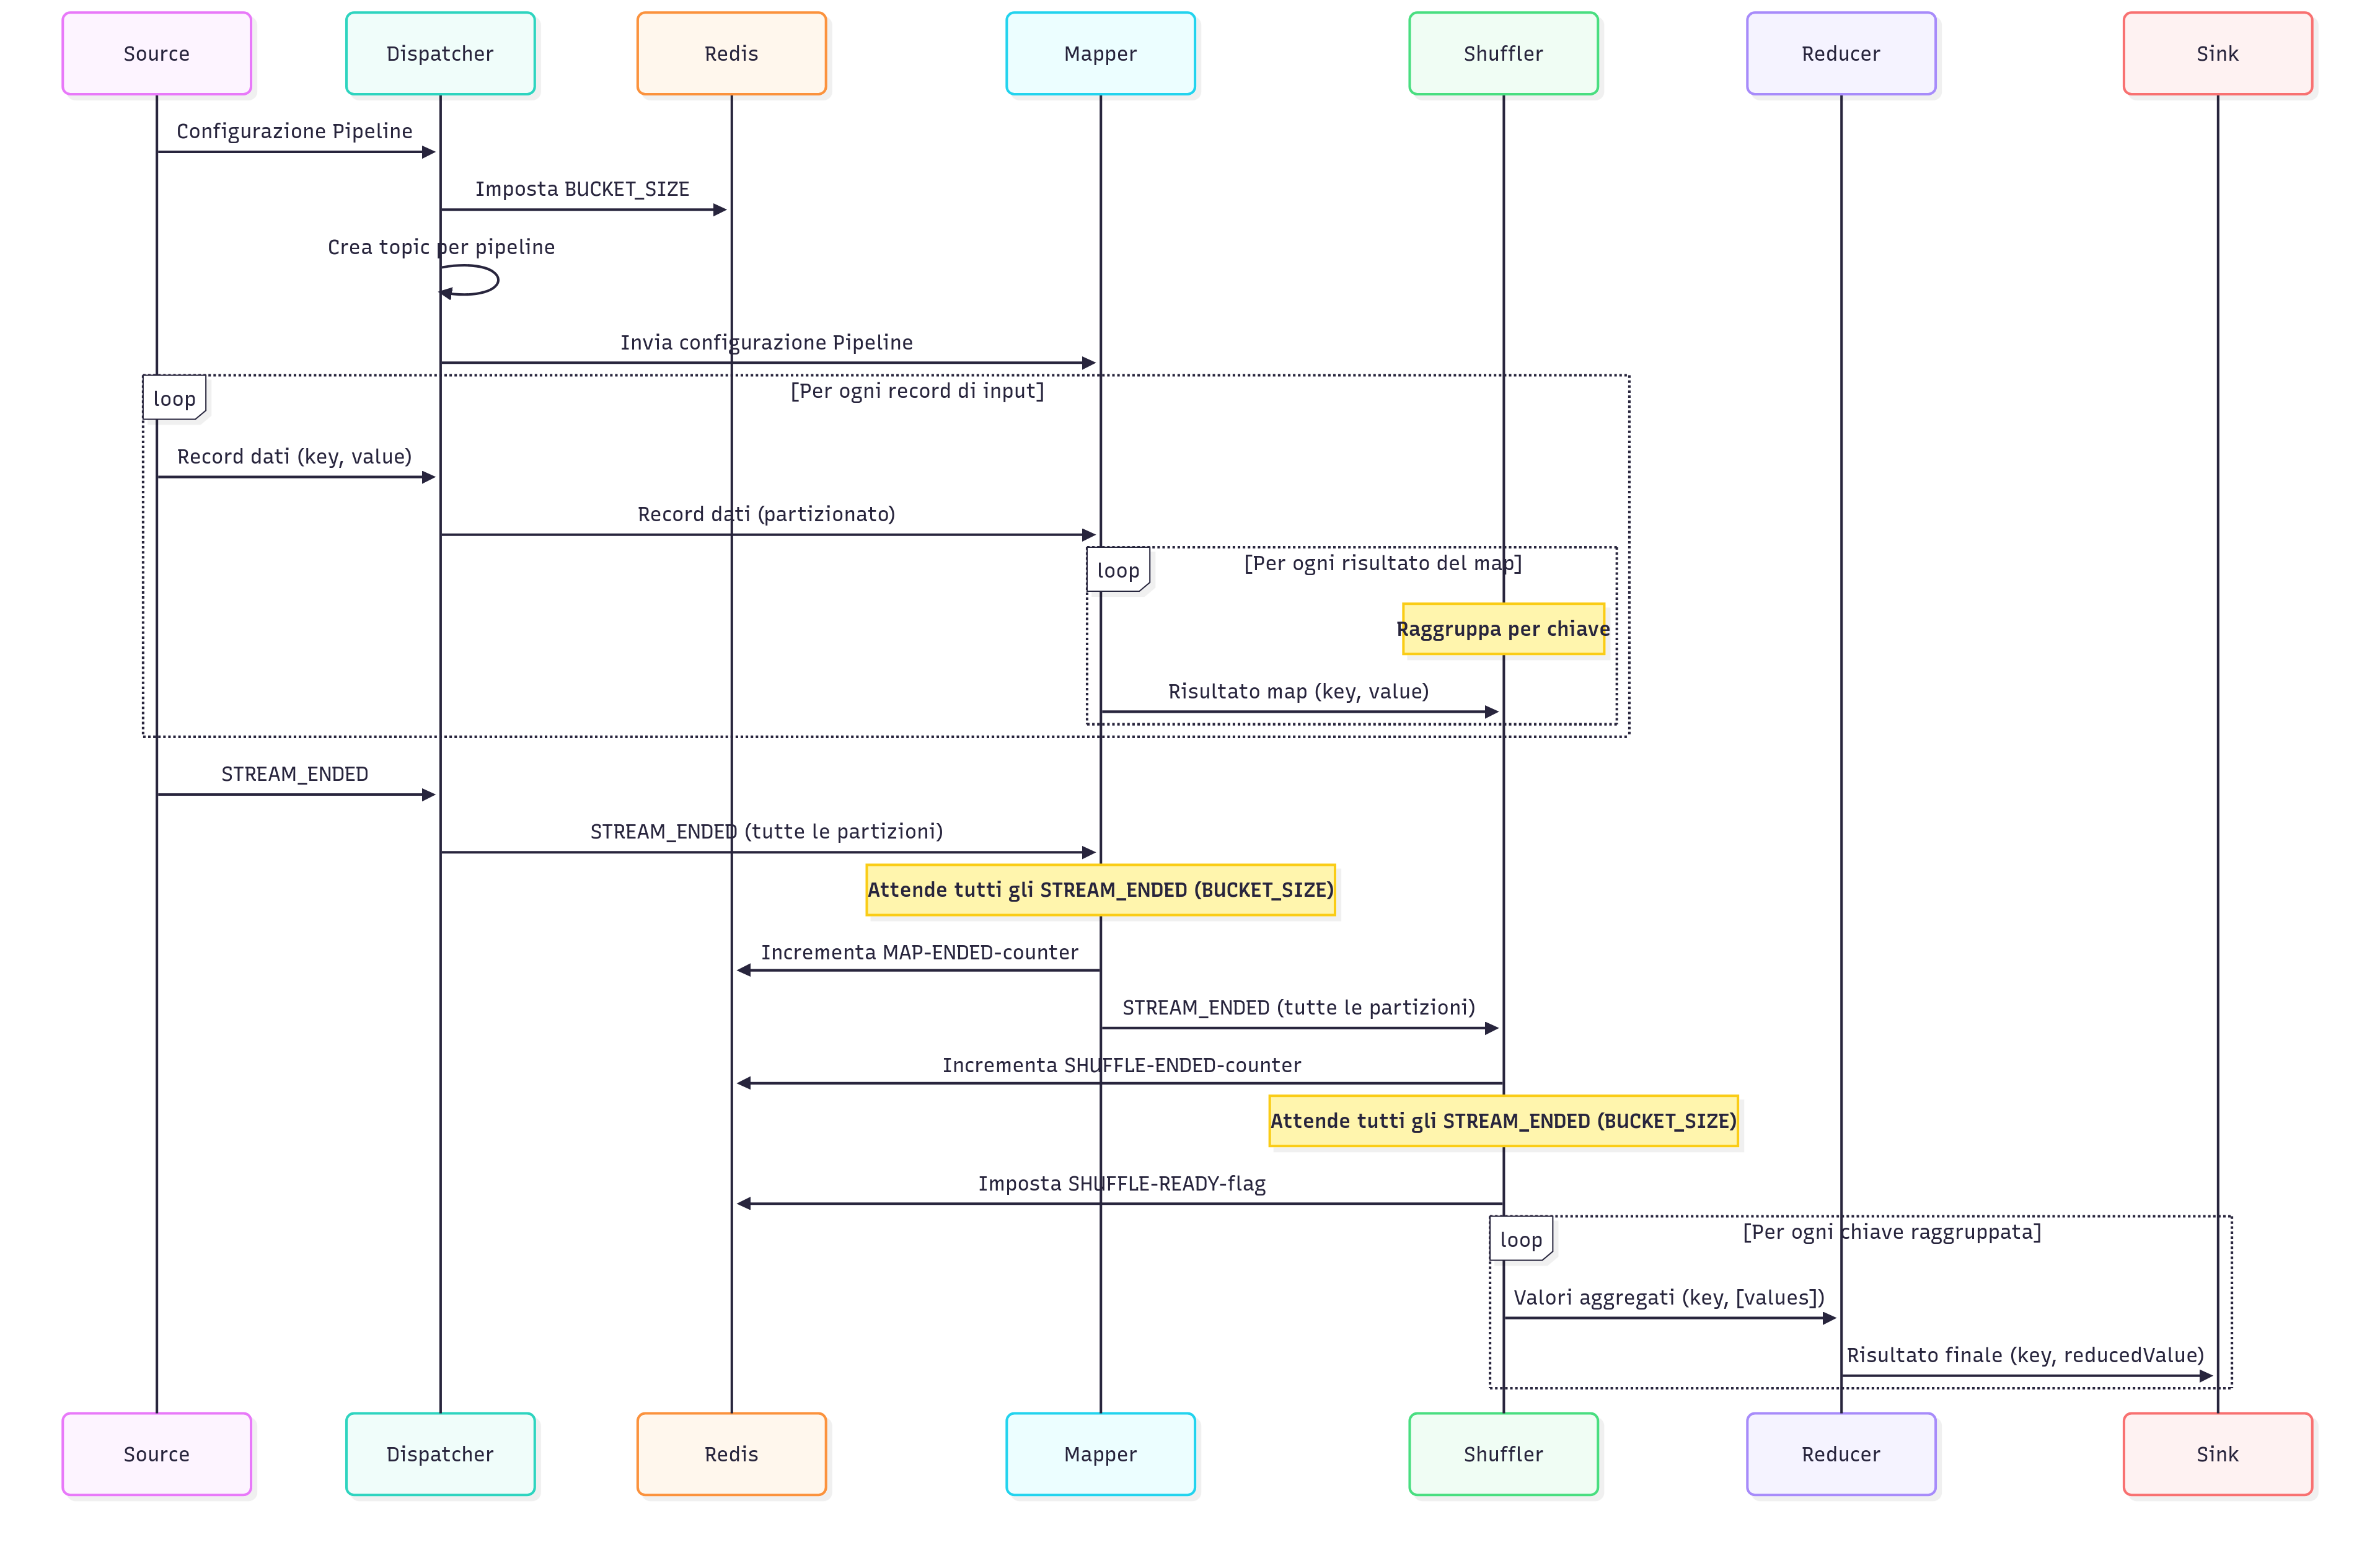
\includegraphics[width=\columnwidth]{images/messagePassing.png}
   \caption{Message passing scheme}
   \label{fig:messagePassing}
\end{figure}

\subsection{Deeper into the stream ending}
\label{sec:streamEnding}

\subsubsection{Mappers}
A mapper receiving its \verb|STREAM_ENDED| message cannot directly propagate it to the shuffle topic, because other mappers may still be processing source records.
% The approach of letting every mapper propagate the \verb|STREAM_ENDED| message to the shuffle topic, and then having the shufflers count how many \verb|STREAM_ENDED| messages they have received, would need a \textbf{shared counter} among shufflers.
The only way I could find to guarantee that all mappers have finished processing is to use a \texttt{redis} \textbf{shared counter}.
When a mapper receives the \verb|STREAM_ENDED| message, it increments the counter in \texttt{redis}.
If the counter equals the number of mappers, then the mapper can propagate the \verb|STREAM_ENDED| message to the shuffle topic.
This is shown in Listing \ref{lst:streamEndedMapper}.\\
A schema in Fig. \ref{fig:redisSynch} wraps up the logic.

\begin{lstlisting}[label={lst:streamEndedMapper}, caption={Handling the STREAM\_ENDED message in a mapper},captionpos={top}]
   // Increment the counter for the number of ended messages
   await redis.incr(`${pipelineID}-MAP-ENDED-counter`);
   
   // Dispatcher sends one STREAM_ENDED message for each map partition, i.e. BUCKET_SIZE times
   // We need to wait for all the STREAM_ENDED messages to arrive before starting to send to shuffle
   const counter = await redis.get(`${pipelineID}-MAP-ENDED-counter`);
   if (!counter || Number(counter) !== BUCKET_SIZE) {
      // In case we have not yet received all the STREAM_ENDED messages, we simply return,
      // as we are not ready to send to shuffle yet, and we have already incremented the counter
      console.log(`[MAP/${WORKER_ID}] Received stream ended message. Got ${counter}/${BUCKET_SIZE} messages... for ${pipelineID}`);
      return;
   }
   else {
      // One of the mappers will receive the last STREAM_ENDED message from the dispatcher
      // and enter this else branch. Here, we propagate the STREAM_ENDED message to the shuffle,
      // One for each partition, i.e. BUCKET_SIZE times
      console.log(`[MAP/${WORKER_ID}] Received last STREAM_ENDED message. `);
   
      // Send to shuffle consumer special value to start feeding the reduce
      // Send onto all partitions
      for (let i = 0; i < BUCKET_SIZE; i++) {
         await producer.send({
            topic: `${SHUFFLE_TOPIC}`,
            messages: [{
               key: `${pipelineID}__${STREAM_ENDED_KEY}`,
               value: JSON.stringify(newStreamEndedMessage(val.pipelineID, null)),
               partition: i,
            }],
         });
      }
      console.log(`[MAP/${WORKER_ID}] Propagated stream ended message to shuffle...`);
\end{lstlisting}


\subsubsection{Shufflers}
The shuffler nodes use similar logic for \verb|STREAM_ENDED| messages. 
They handle standard map records by grouping them by key, but when a \verb|STREAM_ENDED| message is received, they increment a counter in \texttt{redis}. If it's still below the \verb|BUCKET_SIZE| threshold, they do nothing and return.
The shuffler receiving the last \verb|STREAM_ENDED| message sets a \texttt{redis} flag, signaling that the shuffling phase is over, and sends another \verb|STREAM_ENDED| message to all \textit{shuffle} partitions to ``wake up'' the shufflers and have them start sending the \textit{shuffle} records to the \textit{reduce} topic.

\begin{lstlisting}[label={lst:streamEndedShuffler}, caption={Handling the STREAM\_ENDED message in a shuffler},captionpos={top}]
   // Increment the counter for the number of STREAM_ENDED messages
   if (!await redis.get(`${pipelineID}-SHUFFLE-READY-flag`)) {
      await redis.incr(`${pipelineID}-SHUFFLE-ENDED-counter`);
   }
   // If we have not yet received all the STREAM_ENDED messages, we simply return
   const streamEndedCounter = await redis.get(`${pipelineID}-SHUFFLE-ENDED-counter`);
   if (!streamEndedCounter || Number(streamEndedCounter) < BUCKET_SIZE) {
      return;
   }
   // if reached the number of STREAM_ENDED messages, wake everyone with a stream Ended message 
   // having a flag set to make them recognize it as a dummy message
   if (!(await redis.get(`${pipelineID}-SHUFFLE-READY-flag`))) {
      await redis.set(`${pipelineID}-SHUFFLE-READY-flag`, `true`);
      for (let i = 0; i < BUCKET_SIZE; i++) {
         await producer.send({
            topic: `${SHUFFLE_TOPIC}`,
            messages: [{
               key: `${pipelineID}__${STREAM_ENDED_KEY}`,
               value: JSON.stringify(newStreamEndedMessage(val.pipelineID, val.data)),
               partition: i
            }],
         });
      }
   }
  
   // At this point we are ready to send the shuffle records to the reduce topic, all STREAM_ENDED messages have been received
   if (await redis.get(`${pipelineID}-SHUFFLE-READY-flag`)) {
      // Send to REDUCE_TOPIC the shuffle records
\end{lstlisting}

\newpage
\begin{figure}[htbp]
   \centering
   \caption{Scheme wrapping up the redis logic for synchronizing the end of the stream}
   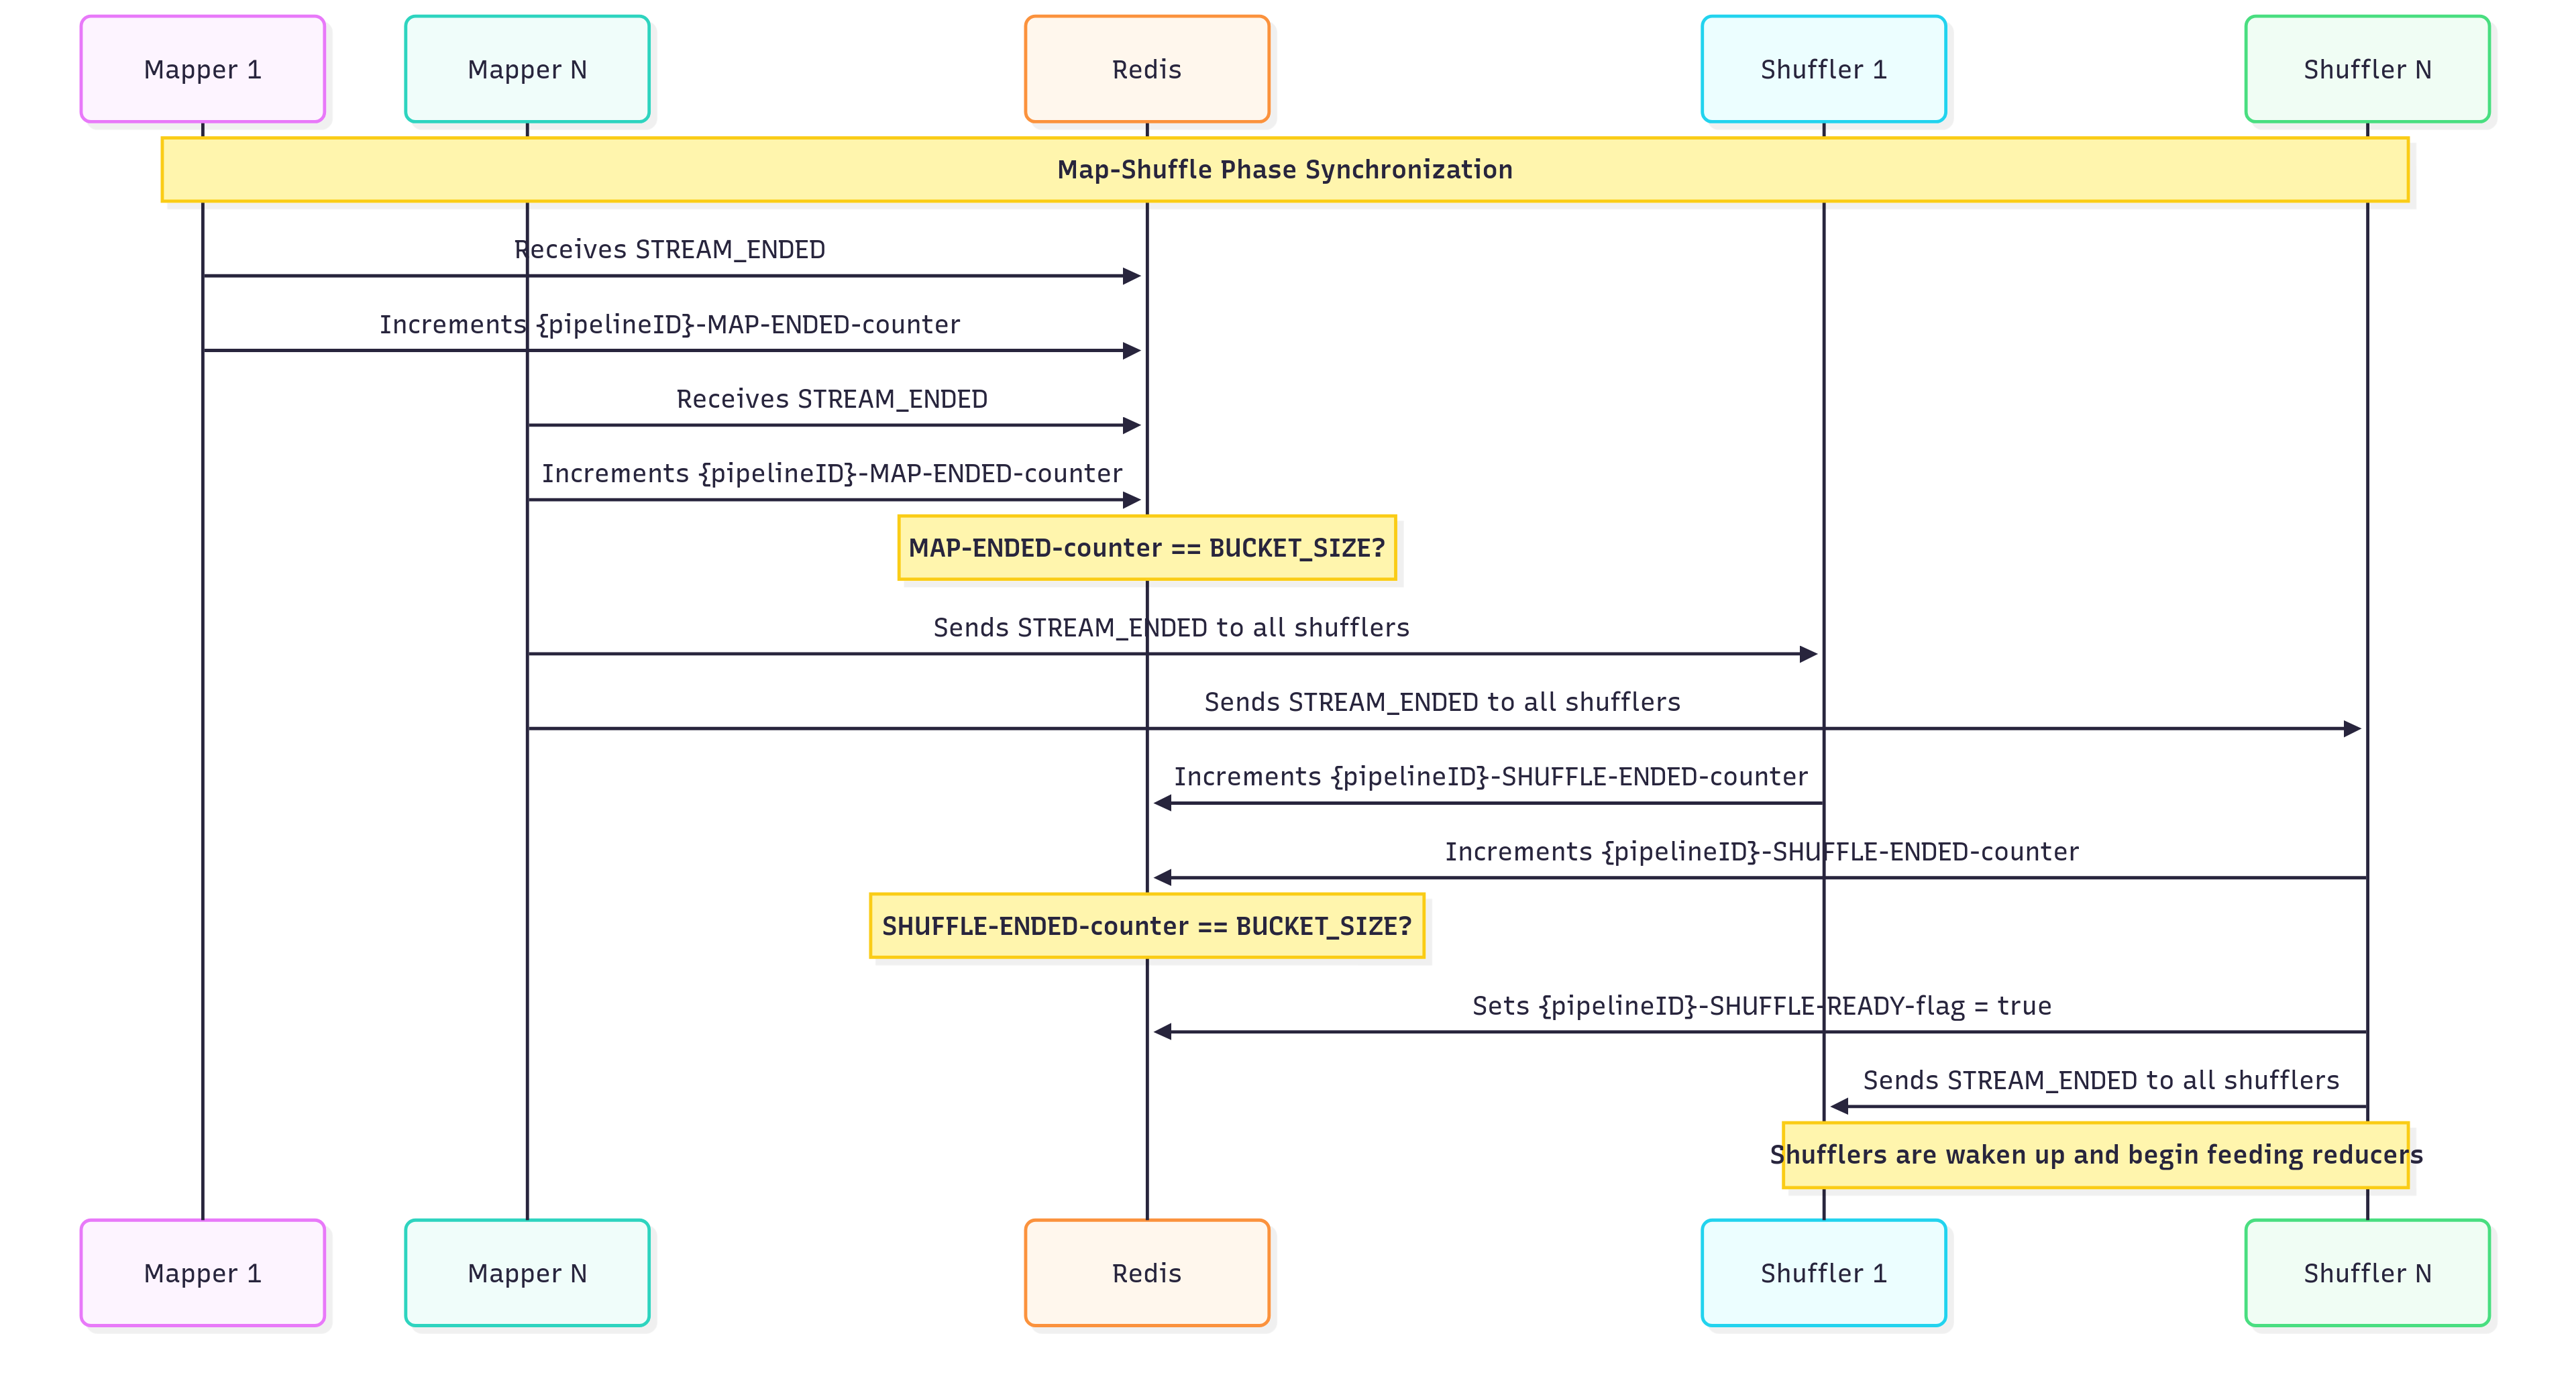
\includegraphics[width=\columnwidth]{images/redisSynch.png}
   \label{fig:redisSynch}
\end{figure}

\subsubsection{Reducers}
The reducer nodes will simply perform the reduce operation on the \textit{shuffle} records they receive and forward the results to the \textit{sink} topic.
No \verb|STREAM_ENDED| messages are needed anymore.

\framedt{Making the sinks know when the stream has ended}{
   Making sink nodes know when the stream has ended would require the same ``messy'' logic as above. Given that the sink nodes are not meant to be used for further processing, but only for outputting the results, and that ideally they should be ``user-defined'', i preferred to let things be simpler.  
}

\section{Conclusions}

Throughout the development, it has been interesting to deal with the issues discussed earlier, especially the \textbf{synchronization} among nodes. Kafka's design naturally avoided the need to handle access to critical code sections or shared data, but some synchronization mechanism over the \textsc{MapReduce} phases was still needed, as the overall process essentially follows the \textsc{BSP} model.\\
The major challenge that may arise with this type of system appears to be message passing and synchronization handling while maintaining scalability and isolation among nodes.\\
An enhancement in the computational performance of a single operation may be negligible or ineffective if not supported by an efficient and robust way to communicate the result of such operation.
In this basic implementation, the Kafka broker acts as the main bottleneck, since it must handle all messages. For very basic operations (such as word counting), the overhead introduced by Kafka's message passing, even if batching is used, may be more significant than the processing itself.

A posteriori, an architecture similar to the adopted one may better suit node clusters that do not have to work as ``sequentially'' as in the \textsc{MapReduce} framework, where the information exchanged among them is less intensive and does not enforce strict process ordering, allowing for better exploitation of Kafka's design while avoiding synchronization delays.\\
Hence, I could observe how an initial poor design choice ---in this case regarding tool selection--- can undermine the success of an implementation, and how potential flaws may be hidden in technical details that are not immediately apparent at first glance.

The aim of the project was to pose challenges whose resolution has led me to gain a deeper understanding of Kafka, MapReduce, TypeScript ---which I had never used before---, and other concepts such as Synchronization and Scalability.

\end{document}